% Diagrama 1: Arquitectura jerárquica de la MANET
% Compilar con: pdflatex arquitectura.tex  (sale arquitectura.pdf)
% Ancho natural ~14.7 cm: se incluye a \textwidth casi sin reducir la letra.
\documentclass[tikz,border=4pt]{standalone}
\usetikzlibrary{arrows.meta}
\usepackage{amsmath}
\begin{document}
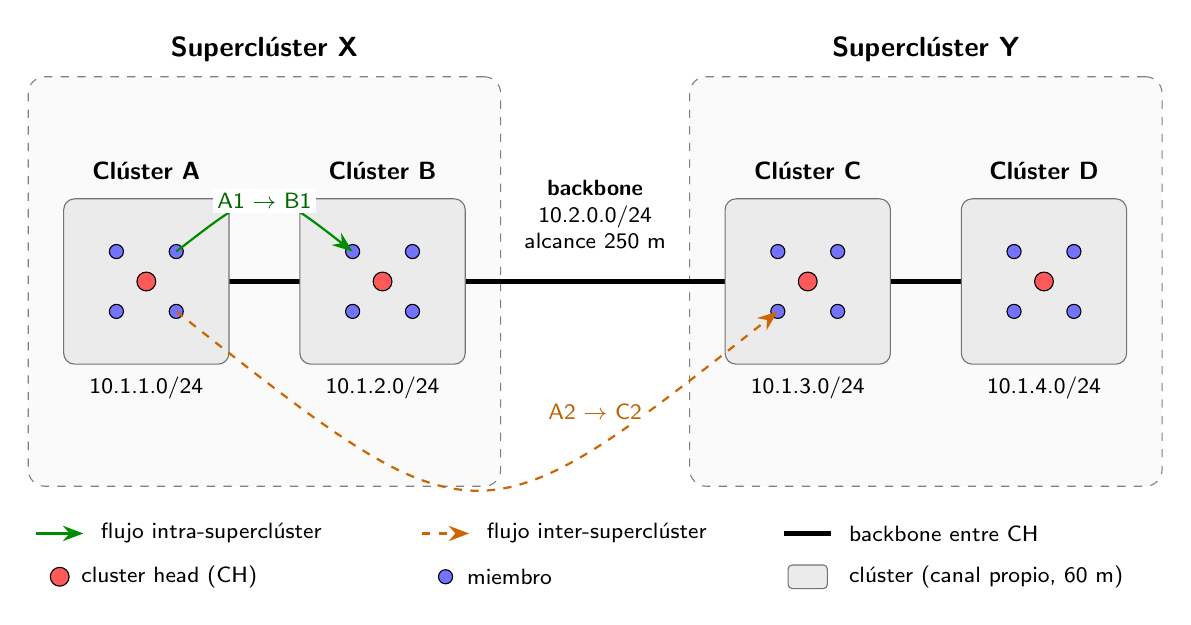
\begin{tikzpicture}[
  font=\sffamily\small,
  super/.style={draw=black!50, dashed, rounded corners=6pt, fill=black!2},
  cluster/.style={draw=black!55, rounded corners=4pt, fill=black!8,
                  minimum width=2.1cm, minimum height=2.1cm},
  ch/.style={circle, draw=black, fill=red!65, inner sep=2.4pt},
  member/.style={circle, draw=black, fill=blue!55, inner sep=1.8pt},
  arr/.style={-{Stealth[length=2.6mm]}},
  etiqueta/.style={fill=white, inner sep=1.5pt, font=\sffamily\footnotesize},
]
% --- Superclústeres -------------------------------------------------------
\node[super, minimum width=6.0cm, minimum height=5.2cm] (X) at (0,0) {};
\node[super, minimum width=6.0cm, minimum height=5.2cm] (Y) at (8.4,0) {};
\node[font=\sffamily\bfseries] at (0,2.95)   {Superclúster X};
\node[font=\sffamily\bfseries] at (8.4,2.95) {Superclúster Y};

% --- Backbone entre CH (detrás de los clústeres) ---------------------------
\draw[black, line width=1.6pt] (-1.5,0) -- (9.9,0);
\node[etiqueta, align=center] at (4.2,0.85)
  {\textbf{backbone}\\10.2.0.0/24\\alcance 250 m};

% --- Clústeres --------------------------------------------------------------
\foreach \cx/\nombre/\red in {-1.5/A/1, 1.5/B/2, 6.9/C/3, 9.9/D/4} {
  \node[cluster] at (\cx,0) {};
  \node[font=\sffamily\small\bfseries] at (\cx,1.4) {Clúster \nombre};
  \node[font=\sffamily\footnotesize] at (\cx,-1.35) {10.1.\red.0/24};
  % CH en el centro y cuatro miembros alrededor
  \node[ch] at (\cx,0) {};
  \foreach \dx/\dy in {0.38/0.38, -0.38/0.38, 0.38/-0.38, -0.38/-0.38}
    \node[member] at (\cx+\dx,\dy) {};
}

% --- Flujo dentro del superclúster X (A1 -> B1) ----------------------------
\draw[green!55!black, thick, arr] (-1.12,0.38) .. controls (0,1.25) .. (1.12,0.38);
\node[etiqueta, text=green!40!black] at (0,1.02) {A1 $\rightarrow$ B1};

% --- Flujo entre superclústeres (A2 -> C2) ---------------------------------
\draw[orange!80!black, thick, dashed, arr]
  (-1.12,-0.38) .. controls (2.7,-3.4) .. (6.52,-0.38);
\node[etiqueta, text=orange!75!black] at (4.2,-1.66) {A2 $\rightarrow$ C2};

% --- Leyenda (dos filas) ----------------------------------------------------
\begin{scope}[font=\sffamily\footnotesize]
  % Fila 1
  \draw[green!55!black, thick, arr] (-2.9,-3.2) -- (-2.3,-3.2);
  \node[right] at (-2.2,-3.2) {flujo intra-superclúster};
  \draw[orange!80!black, thick, dashed, arr] (2.0,-3.2) -- (2.6,-3.2);
  \node[right] at (2.7,-3.2) {flujo inter-superclúster};
  \draw[black, line width=1.6pt] (6.6,-3.2) -- (7.2,-3.2);
  \node[right] at (7.3,-3.2) {backbone entre CH};
  % Fila 2
  \node[ch] at (-2.6,-3.75) {};
  \node[right] at (-2.45,-3.75) {cluster head (CH)};
  \node[member] at (2.3,-3.75) {};
  \node[right] at (2.45,-3.75) {miembro};
  \draw[draw=black!55, rounded corners=1.5pt, fill=black!8] (6.65,-3.9) rectangle (7.15,-3.6);
  \node[right] at (7.3,-3.75) {clúster (canal propio, 60 m)};
\end{scope}
\end{tikzpicture}
\end{document}
